\documentclass[11pt]{article}
\usepackage[margin=0.85in]{geometry}
\usepackage[T1]{fontenc}
\usepackage{amsmath,amssymb,booktabs,graphicx,xurl,hyperref}
\graphicspath{{outputs/task1/}{outputs/task2/}{outputs/task3/debug/}{outputs/task3/lego_train/}{outputs/task3/lego_train/validation/}{outputs/task3/lego_train/mesh/}}
\hypersetup{pdftitle={CS 498 HW4 Report},pdfauthor={Siddharth Dinkar}}
\setlength{\parindent}{0pt}
\setlength{\parskip}{4pt}
\renewcommand{\topfraction}{0.9}
\renewcommand{\bottomfraction}{0.9}
\renewcommand{\textfraction}{0.05}
\renewcommand{\floatpagefraction}{0.85}
\setcounter{topnumber}{3}
\setcounter{totalnumber}{5}

\title{\vspace{-0.6in}CS 498 HW4 Report\\Tiny NeRF for Novel View Synthesis}
\author{Siddharth Dinkar (sdinkar2)}
\date{Fall 2026\vspace{-0.15in}}

\begin{document}
\maketitle

\section{Rays and positional encoding}

The camera sits at the origin of its own frame and looks along $-z$, with $x$ to the right and $y$ up. For an image of height $H$ and width $W$ with focal length $f$ in pixels, the pixel in column $i$ and row $j$ gets the camera-space direction
\[
\mathbf{d}_{\mathrm{cam}} = \left[\frac{i - W/2}{f},\; -\frac{j - H/2}{f},\; -1\right]^{\top}.
\]
With the camera-to-world rotation $R$ and the camera center $\mathbf{o}$ taken from the pose matrix, the world-space ray is
\[
\mathbf{r}(t) = \mathbf{o} + t\,\mathbf{d}, \qquad \mathbf{d} = R\,\mathbf{d}_{\mathrm{cam}}.
\]
Every pixel shares the origin $\mathbf{o}$, so the origin is broadcast to $[H, W, 3]$. The rotation is applied to the whole $[H, W, 3]$ direction grid in one product with $R^{\top}$ on the right, which gives $R\,\mathbf{d}_{\mathrm{cam}}$ at every pixel.

The row index $j$ grows downward in the image while camera $y$ points up, so the $y$ component carries a minus sign. Without it the rendered image would be flipped vertically. Directions stay unnormalized so that the third camera-space component is exactly $-1$. The ray parameter $t$ then equals depth along the optical axis, and the near and far bounds of 2 and 6 describe the same two planes for every pixel. The renderer recovers true distances by multiplying depth gaps by $\lVert\mathbf{d}\rVert_2$.

Positional encoding maps an input $\mathbf{x}$ with $D$ coordinates to
\[
\gamma(\mathbf{x}) = \left[\mathbf{x},\, \sin(2^{0}\mathbf{x}),\, \cos(2^{0}\mathbf{x}),\, \ldots,\, \sin(2^{L-1}\mathbf{x}),\, \cos(2^{L-1}\mathbf{x})\right],
\]
which has width $D(1 + 2L)$. The full run uses $L = 8$ for positions, giving $3 \times 17 = 51$ features, and $L = 4$ for view directions, giving $3 \times 9 = 27$ features.

\begin{figure}[htbp]
\centering
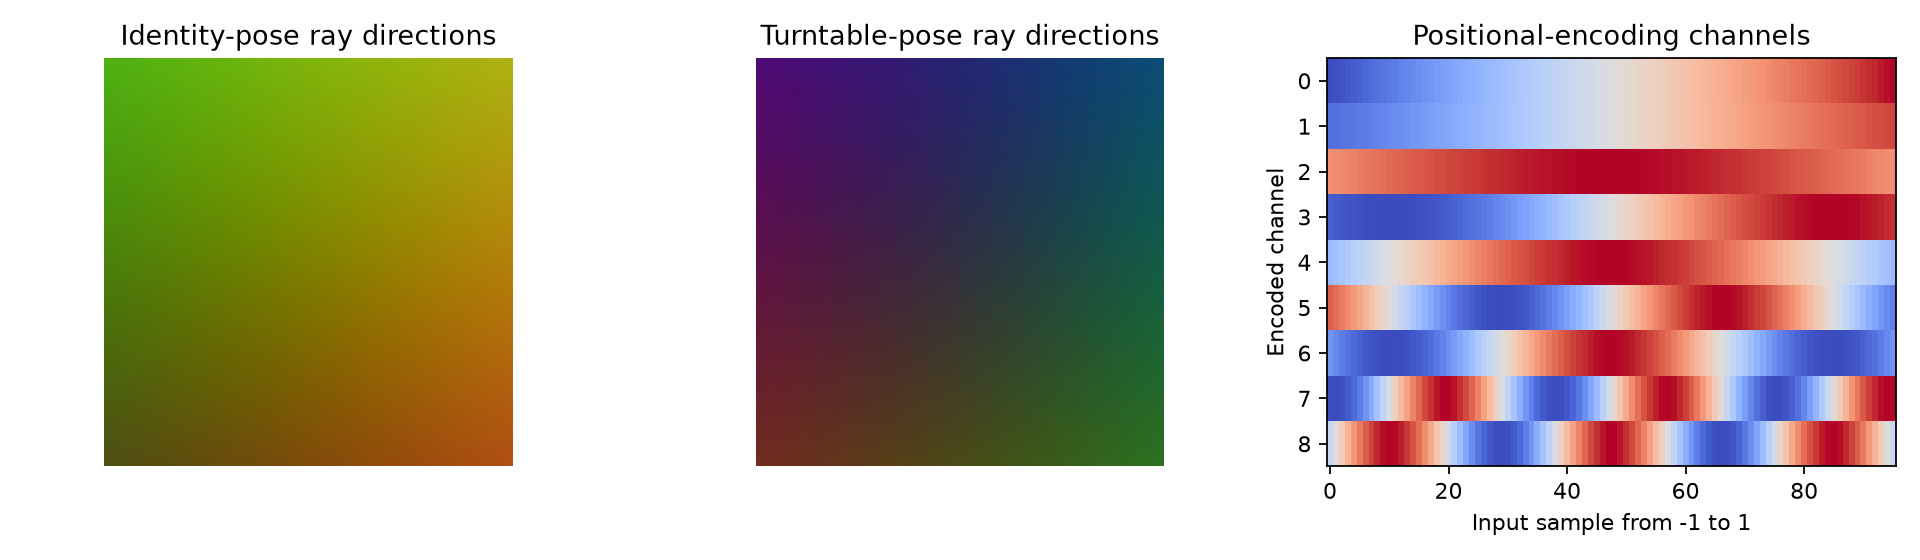
\includegraphics[width=0.74\linewidth]{outputs/task1/task1_visual_checkpoint.png}
\caption{Task 1 visual checkpoint. Ray directions shown as colors for the identity pose and for a turntable pose, and the nine encoding channels of a one-dimensional input with $L = 4$.}
\label{fig:task1}
\end{figure}

In Figure~\ref{fig:task1} both ray panels vary smoothly with no seams or flips. The turntable pose changes the colors because the same camera-space directions are rotated into a different world orientation. The encoding panel shows the raw input in channel 0, followed by sine and cosine pairs whose frequency doubles from one pair to the next.

\section{Tiny NeRF and volume rendering}

The network takes the 51-dimensional encoded position and the 27-dimensional encoded view direction. Six linear layers of width 128 process the position, each followed by ReLU. Before layer 3, counting from zero, the current 128-dimensional activation is concatenated with the original encoded position, so that layer receives 179 inputs. This skip connection gives the later layers direct access to the input coordinates. The density head maps the final point feature to one raw density value. Density is computed before the view direction enters the network, so it depends on position only. For color, a feature head maps the same point feature to 128 dimensions with no activation, the encoded direction is concatenated to give 155 dimensions, a view layer with ReLU reduces this to 64, and the RGB head outputs three raw color values. The forward pass returns $[c^{\mathrm{raw}}_r, c^{\mathrm{raw}}_g, c^{\mathrm{raw}}_b, \sigma^{\mathrm{raw}}]$ with no output activation. The renderer applies the sigmoid and the ReLU.

For $S$ samples per ray the base depths are
\[
\bar{z}_s = z_{\mathrm{near}} + \frac{s}{S-1}\,(z_{\mathrm{far}} - z_{\mathrm{near}}), \qquad s = 0, \ldots, S-1.
\]
With perturbation, the midpoints $m_s = \tfrac{1}{2}(\bar{z}_s + \bar{z}_{s+1})$ split the range into $S$ strata. The first stratum starts at $z_{\mathrm{near}}$ and the last ends at $z_{\mathrm{far}}$. Each ray draws one independent sample per stratum,
\[
z_{n,s} = \ell_s + \epsilon_{n,s}\,(u_s - \ell_s), \qquad \epsilon_{n,s} \sim \mathcal{U}[0, 1),
\]
where $\ell_s$ and $u_s$ are the lower and upper bounds of stratum $s$. The strata do not overlap, so the depths stay ordered without sorting. Sample points are $\mathbf{x}_{n,s} = \mathbf{o}_n + z_{n,s}\,\mathbf{d}_n$.

For compositing, color and density are activated as $\mathbf{c} = \mathrm{sigmoid}(\mathbf{c}^{\mathrm{raw}})$ and $\sigma = \mathrm{ReLU}(\sigma^{\mathrm{raw}})$. The distance covered by sample $s$ is $\delta_{n,s} = (z_{n,s+1} - z_{n,s})\,\lVert\mathbf{d}_n\rVert_2$, with a final interval of $10^{10}$. Then
\[
\alpha_{n,s} = 1 - e^{-\sigma_{n,s}\delta_{n,s}}, \qquad
T_{n,s} = \prod_{j<s}\left(1 - \alpha_{n,j} + 10^{-10}\right), \qquad
w_{n,s} = T_{n,s}\,\alpha_{n,s},
\]
\[
\mathbf{C}_n = \sum_s w_{n,s}\,\mathbf{c}_{n,s}, \qquad
D_n = \sum_s w_{n,s}\,z_{n,s}, \qquad
A_n = \sum_s w_{n,s}.
\]
The transmittance product is exclusive. I compute it by prepending a column of ones, taking a cumulative product, and dropping the last column. The weights are not renormalized. With a white background the remaining transparency $1 - A_n$ is added to each channel of $\mathbf{C}_n$.

\begin{figure}[htbp]
\centering
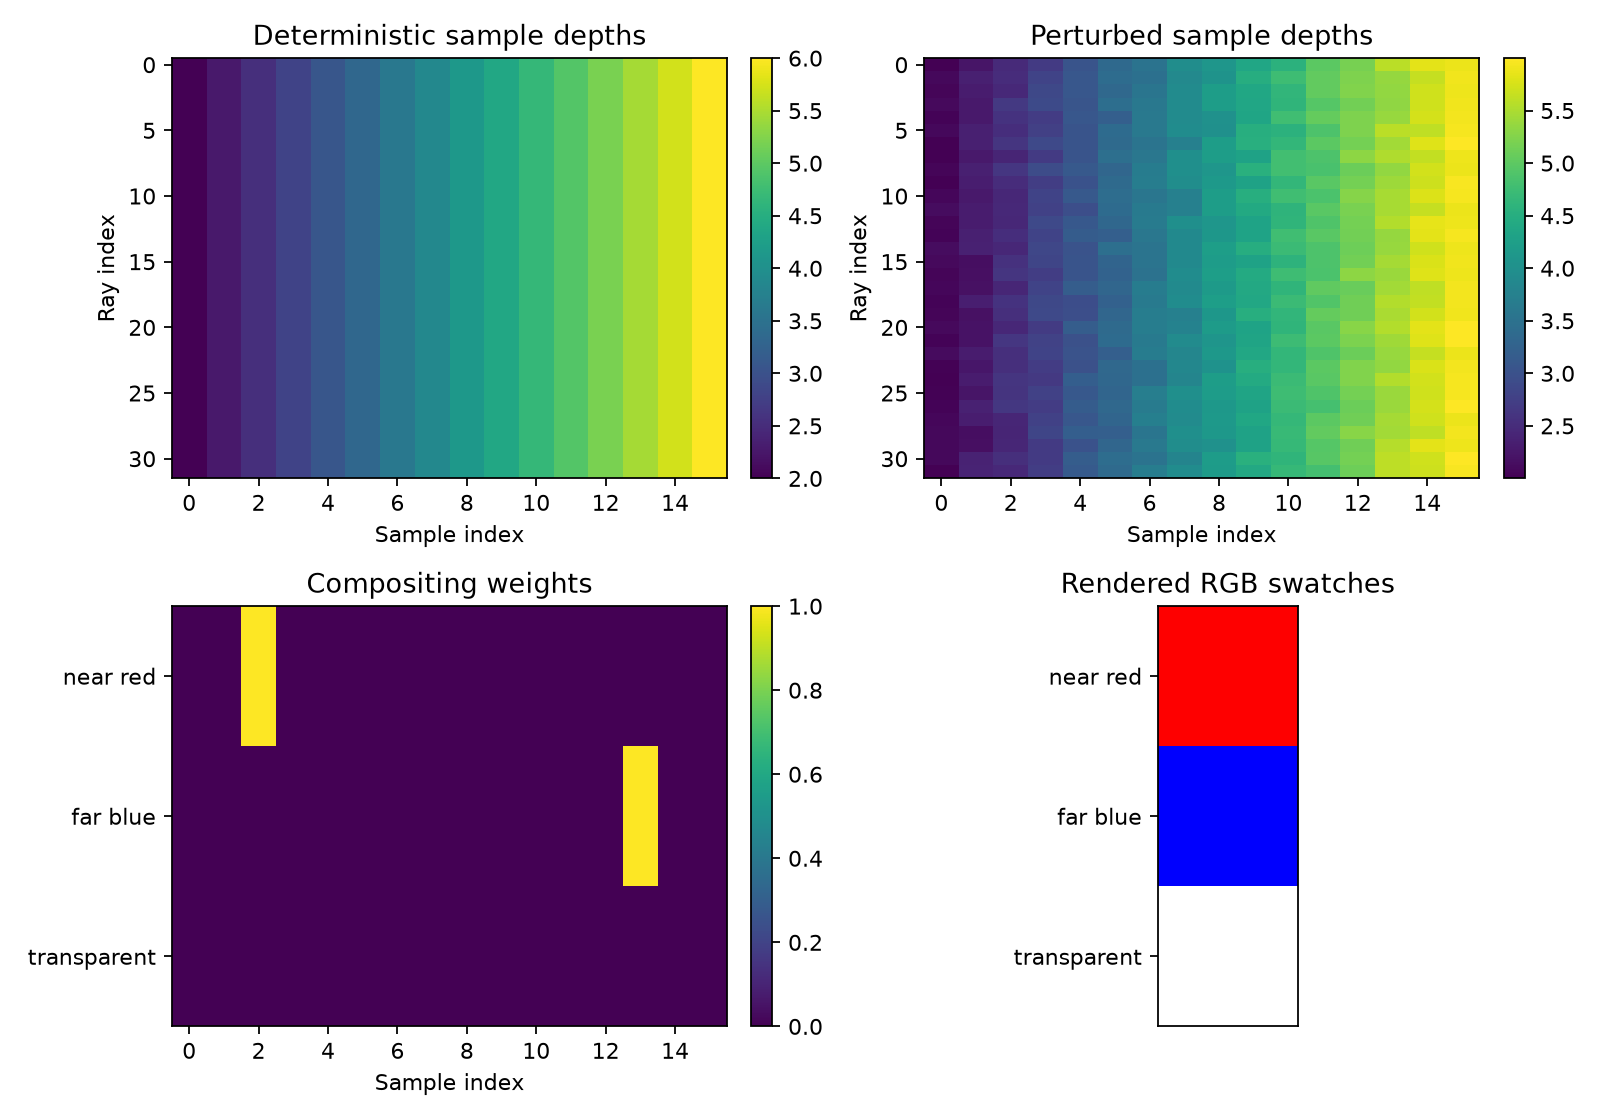
\includegraphics[width=0.5\linewidth]{outputs/task2/task2_visual_checkpoint.png}
\caption{Task 2 visual checkpoint. Top: deterministic and perturbed sample depths for 32 rays with 16 samples. Bottom: compositing weights and rendered colors for three synthetic rays.}
\label{fig:task2}
\end{figure}

In the deterministic panel of Figure~\ref{fig:task2} every row is identical and the depths increase evenly from 2 to 6. In the perturbed panel the rows differ from one another, each row still increases from left to right, and all values stay between 2 and 6. The near red ray has one dense red sample at index 2. That sample receives a weight close to 1 and the ray renders as RGB $[0.998, 0.003, 0.003]$ with depth 1.400 and opacity 1.000. The far blue ray has its dense sample at index 13 and renders as $[0.003, 0.003, 0.998]$ with depth 3.599. The transparent ray has zero weight at every sample, opacity 0.000, and renders the white background.

\section{Training and held-out reconstruction}

The smoke run completed. It trained for 100 steps on images downscaled to $100 \times 100$ with the reduced network, and its logged training PSNR rose from 9.61 dB at step 1 to 10.80 dB at step 100.

The full run trained for 10{,}000 iterations with Adam at learning rate $5 \times 10^{-4}$ and a mean squared error loss on RGB. Each batch holds 1{,}024 rays drawn at random from the 50 training images at $200 \times 200$, with 64 stratified samples per ray.

\begin{figure}[htbp]
\centering
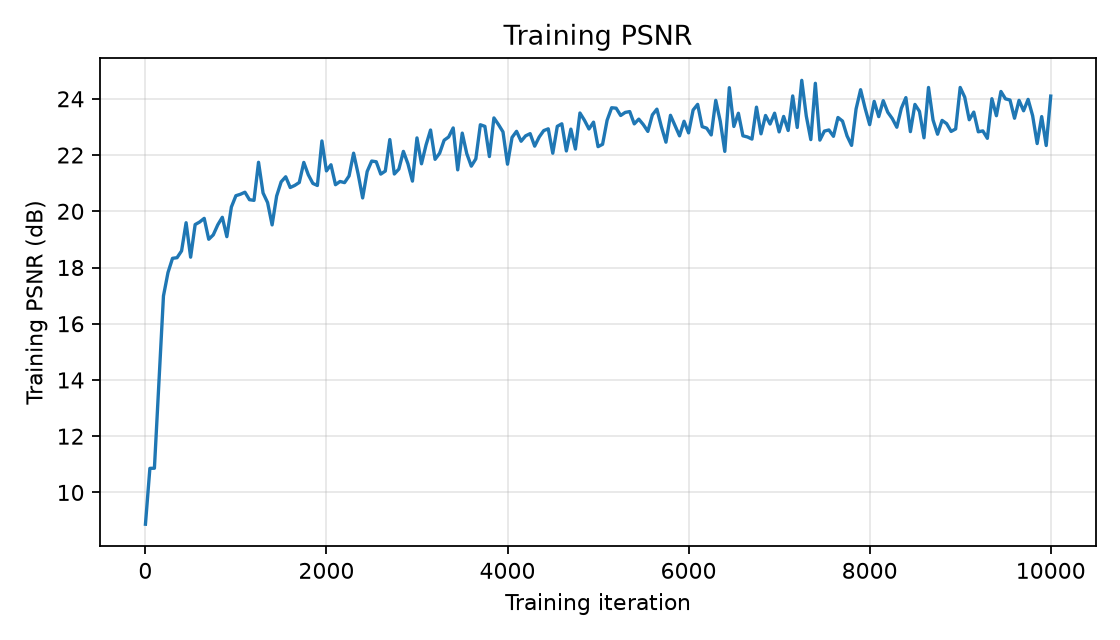
\includegraphics[width=0.42\linewidth]{outputs/task3/lego_train/train_psnr_curve.png}\hfill
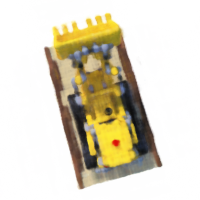
\includegraphics[width=0.22\linewidth]{outputs/task3/lego_train/val_010000_view_00.png}\hfill
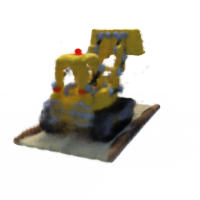
\includegraphics[width=0.22\linewidth]{outputs/task3/lego_train/val_010000_view_01.png}
\caption{Training PSNR over 10{,}000 iterations and the two milestone renders at step 10{,}000.}
\label{fig:train}
\end{figure}

The curve in Figure~\ref{fig:train} rises quickly to 19.59 dB by step 450 and then climbs slowly, with batch-to-batch noise of about 1 dB. The final logged training PSNR is 24.10 dB at step 10{,}000. Both milestone renders show a recognizable bulldozer with the bucket, cab, tracks, and base plate in the right places.

\begin{table}[htbp]
\centering
\begin{tabular}{lcccccc}
\toprule
Validation view & 0 & 1 & 2 & 3 & 4 & Mean \\
\midrule
PSNR in dB & 23.25 & 24.37 & 24.54 & 24.93 & 24.07 & 24.23 \\
SSIM & 0.855 & 0.879 & 0.858 & 0.858 & 0.839 & 0.858 \\
\bottomrule
\end{tabular}
\caption{Held-out validation metrics from \texttt{validation\_metrics.csv}.}
\label{tab:val}
\end{table}

Mean validation PSNR is 24.23 dB and mean SSIM is 0.858 over the five validation views, as listed in Table~\ref{tab:val}. The validation mean is close to the final training PSNR, so the model reaches about the same quality on unseen poses as on training rays.

\begin{figure}[htbp]
\centering
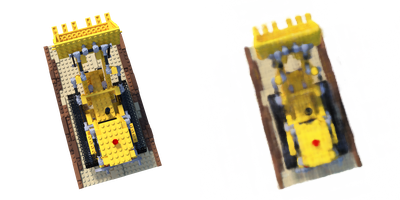
\includegraphics[width=0.42\linewidth]{outputs/task3/lego_train/validation/view_00_comparison.png}
\caption{Validation view 0. Ground truth on the left and the NeRF render on the right.}
\label{fig:val}
\end{figure}

\begin{figure}[htbp]
\centering
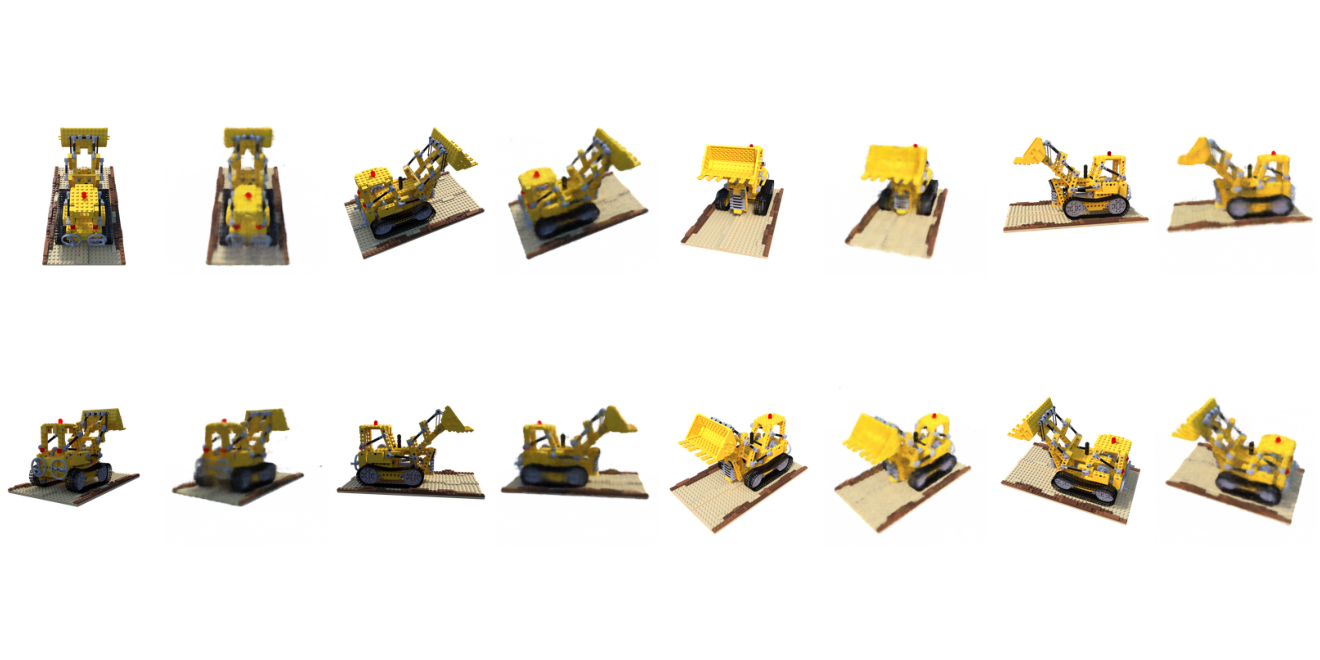
\includegraphics[width=0.82\linewidth,trim=0 55 0 45,clip]{outputs/task3/lego_train/turntable_contact_sheet.png}
\caption{Eight of the twelve held-out turntable views. Each pair shows ground truth on the left and the NeRF render on the right.}
\label{fig:turntable}
\end{figure}

In Figure~\ref{fig:turntable} the pose, scale, and coarse geometry agree in every pair, and the appearance changes smoothly from one view to the next.

The main visible limitation is blur. In Figure~\ref{fig:val} the studs on the base plate and on the yellow bricks are smoothed away, and the gaps in the track treads and the thin struts of the bucket arm are faint or missing. The silhouette is also slightly soft, with a faint halo where the model meets the white background. Validation view 0 looks down on the stud pattern and has the lowest PSNR at 23.25 dB, while view 3 has the highest at 24.93 dB.

\section{Density grid and textured mesh}

The density grid covers $[-1.5, 1.5]^3$ at resolution $96^3$, which is 884{,}736 query points. My function builds the coordinates with \texttt{torch.linspace} and \texttt{torch.meshgrid} using \texttt{ij} indexing so that the axes are ordered $x$, $y$, $z$. It queries the network in chunks of 8{,}192 points in evaluation mode without gradients, passes one fixed unit direction $[0, 0, -1]$ to the color branch, keeps the ReLU of the raw density channel, and restores the previous training mode afterward.

The provided pipeline extracts the surface at density threshold 20 with marching cubes. The visual hull cleanup kept 63{,}667 voxels that are supported by all 50 training masks. After component cleanup the mesh has 22{,}898 vertices and 46{,}084 faces. UV unwrapping splits vertices along chart seams, so the exported files contain 36{,}322 vertices with the same 46{,}084 faces. The texture atlas is $256 \times 256$, and 40{,}037 of its texels are covered.

\begin{figure}[htbp]
\centering
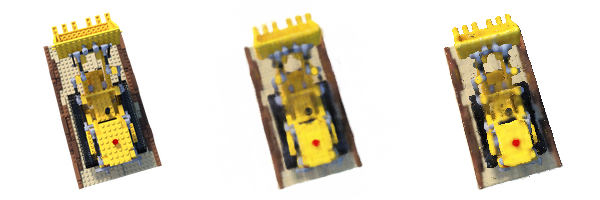
\includegraphics[width=0.49\linewidth]{outputs/task3/lego_train/mesh/view_00_comparison.png}\hfill
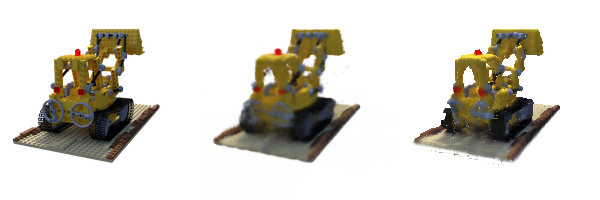
\includegraphics[width=0.49\linewidth]{outputs/task3/lego_train/mesh/view_01_comparison.png}
\caption{Mesh comparisons for view 0 on the left and view 1 on the right. Each triple shows ground truth, the direct NeRF render, and the textured mesh render.}
\label{fig:mesh}
\end{figure}

\begin{table}[htbp]
\centering
\begin{tabular}{lcccc}
\toprule
 & \multicolumn{2}{c}{Direct NeRF} & \multicolumn{2}{c}{Textured mesh} \\
\cmidrule(lr){2-3}\cmidrule(lr){4-5}
View & PSNR in dB & SSIM & PSNR in dB & SSIM \\
\midrule
0 & 23.25 & 0.855 & 21.46 & 0.832 \\
1 & 24.37 & 0.879 & 21.60 & 0.851 \\
Mean & 23.81 & 0.867 & 21.53 & 0.842 \\
\bottomrule
\end{tabular}
\caption{Matched-view metrics against ground truth from \texttt{mesh/comparison.csv}.}
\label{tab:mesh}
\end{table}

Table~\ref{tab:mesh} gives mean direct NeRF values of 23.81 dB and 0.867, and mean textured mesh values of 21.53 dB and 0.842. The mesh stays aligned with both cameras and keeps the main geometry of the bulldozer.

Two differences are visible in Figure~\ref{fig:mesh}. First, the mesh has a hard opaque boundary. Structures thinner than one voxel, which is about 0.032 world units, fall below the threshold in places. In view 1 the edge of the base plate is ragged and small pieces of the base and tracks are missing, while the volume rendering keeps those regions as soft partial coverage. Second, the mesh color is a single baked texture. Each texel stores one color queried from the NeRF, so the mesh has no view dependence and its detail is limited by the atlas resolution. This shows up as dark blotches around the tracks and under the cab in view 1.

\section{Limitations and reproducibility}

All final outputs were generated on the Illinois Campus Cluster through Slurm on one NVIDIA A10 GPU with 4 CPU cores and 16 GB of memory, using Python 3.11 and PyTorch 2.15.0 with CUDA. The seed is 0 from the provided configuration. The full pipeline took 2 minutes 52 seconds of wall time. The commands, run from the \texttt{hw4} directory inside batch jobs, were:

{\small
\begin{verbatim}
python -m unittest tests.test_task1_rays_encoding \
    tests.test_task2_nerf_rendering tests.test_task3_mesh
python task1_rays_encoding.py
python task2_nerf_rendering.py
python task3_train_mesh.py --mode check
python task3_train_mesh.py --mode smoke --device cuda
python task3_train_mesh.py --mode all
python bonus_ball_insertion.py --mode render \
    --checkpoint outputs/task3/lego_train/model.pt
\end{verbatim}
}

The first limitation is model capacity and sampling. The network has six layers of width 128 and each ray uses 64 stratified samples with no second pass that concentrates samples near surfaces. Fine detail such as studs and thin struts is blurred, and validation PSNR stays near 24 dB.

The second limitation is the mesh extraction. A single density threshold on a $96^3$ grid cannot represent structures thinner than a voxel, so thin parts are either lost or thickened. The result also depends on the visual hull cleanup, which needs the training masks, and the baked texture discards view-dependent color.

A further limitation is scope. The model is optimized for one synthetic scene at $200 \times 200$ with known camera poses and a white background, and it must be retrained for any other scene.

\section*{Optional ball-insertion bonus}

The sphere uses the supplied parameters: center $[0.00, -1.20, -0.18]$, radius 0.35, albedo $[0.08, 0.62, 0.24]$, and light direction $[-0.45, -0.65, 1.00]$. The provided code finds the hit depth $t_{b,n}$ of each ray and shades the sphere at the hit point.

For a ray that hits the sphere, my function keeps only the NeRF samples strictly in front of the hit and computes
\[
\mathbf{C}_{\mathrm{front},n} = \sum_{z_{n,s} < t_{b,n}} w_{n,s}\,\mathbf{c}_{n,s}, \qquad
A_{\mathrm{front},n} = \sum_{z_{n,s} < t_{b,n}} w_{n,s}, \qquad
T_{b,n} = \mathrm{clamp}(1 - A_{\mathrm{front},n},\, 0,\, 1),
\]
\[
\mathbf{C}_{\mathrm{insert},n} = \mathbf{C}_{\mathrm{front},n} + T_{b,n}\,\mathbf{c}_{\mathrm{ball},n}.
\]
Rays that miss the sphere keep the original NeRF color and report zero visibility. The sphere is opaque, so samples behind it contribute nothing.

\begin{figure}[htbp]
\centering
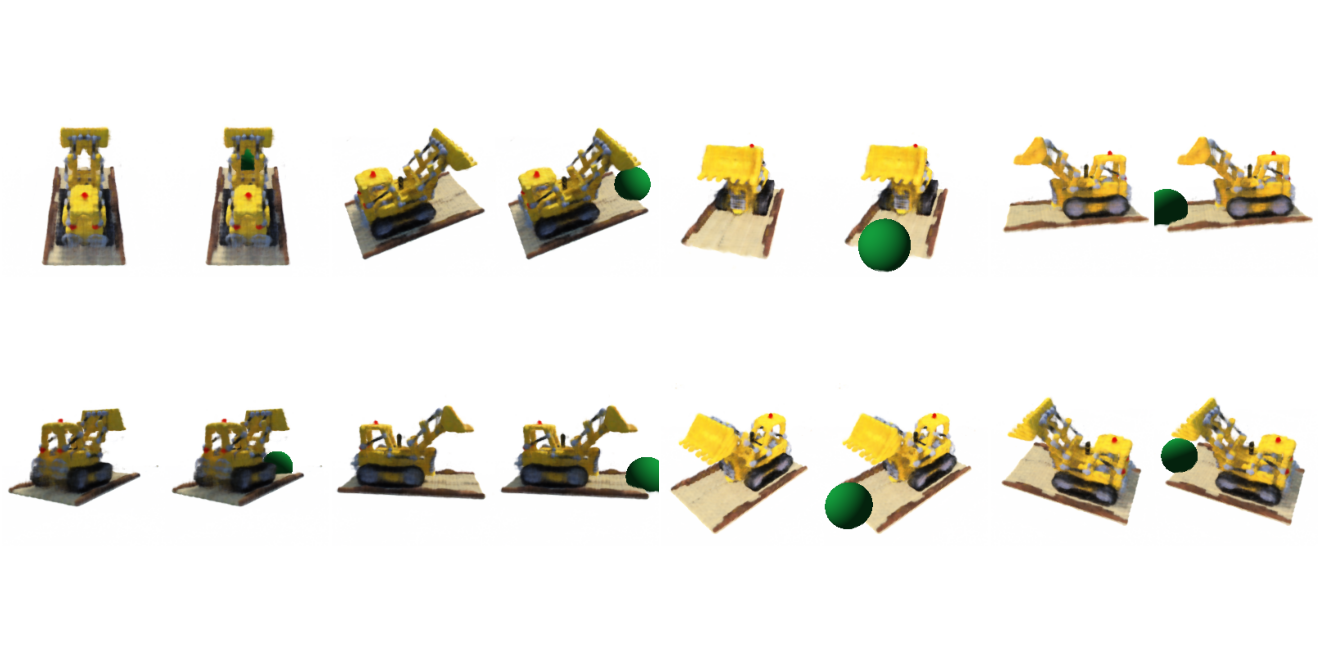
\includegraphics[width=0.74\linewidth,trim=0 55 0 45,clip]{outputs/task3/lego_train/ball_insertion_contact_sheet.png}\hfill
\raisebox{0.04\linewidth}{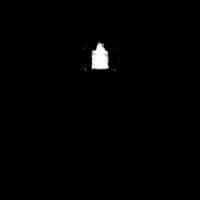
\includegraphics[width=0.2\linewidth]{outputs/task3/lego_train/ball_visibility.png}}
\caption{Left: eight held-out views, each shown as the scene alone and the scene with the inserted sphere. Right: sphere visibility $T_b$ for the first view.}
\label{fig:ball}
\end{figure}

Two views in Figure~\ref{fig:ball} have different occlusion relationships. In the first view of the top row the sphere sits behind the bulldozer arms, and only a small patch is visible through the gap between them. In the third view of the top row the sphere is closer to the camera than the model, is fully visible, and covers part of the base plate.

Expected depth is not sufficient as a z-buffer for two reasons. It is a weighted average of sample depths along the whole ray. On a ray through a soft edge, part of the weight lies in front of the sphere and part lies behind it, and the average can fall on either side of the hit depth. A depth test against that single value makes the pixel either fully sphere or fully scene. The visibility image for the first view contains intermediate gray values along the edges of the visible patch, which a binary depth test cannot produce. In addition, the weights are not renormalized, so a ray with low opacity has an expected depth biased toward zero. A fully transparent ray has depth 0.000, as in the Task 2 checkpoint, and a depth test would wrongly place the empty scene in front of the sphere. The transmittance rule avoids both problems because it uses the fraction of light that reaches the sphere.

\section*{AI-use declaration}
Check one statement.

\begin{itemize}
  \item[$\square$] I did not use generative AI for this homework.
  \item[$\boxtimes$] I used generative AI only in ways explicitly allowed by
  the course policy. Tool/model, purpose, and affected files:
  Claude Opus 5.5 used on the \path{bonus_ball_insertion.py} since AI usage is allowed on the bonus points portions by the course policy like the previous homeworks.
\end{itemize}

I confirm that the submitted code, outputs, numerical results, and written
analysis comply with the course collaboration and AI-use policy.

\end{document}
